\section{Extended Rosenbrock function}
\label{sec:extended_rosenbrock_results}

The extended Rosenbrock function is a generalization of the Rosenbrock function to $n$ dimensions, defined as follows.
Figure \ref{fig:extended_rosenbrock_surf} shows the surface plot of the 2-dimensional extended Rosenbrock function: notice that for $n=2$ it is identical to the standard Rosenbrock function, except for the $\frac12$ term.
\begin{align}
\label{eq:extended_rosenbrock}
F(x) &= \frac12 \sum_{k=1}^n f_k^2(x), &
f_k(x) &= \left \{ \begin{array}{ll}
10(x_k^2 - x_{k+1}), & k\mod 2 = 1\\
x_{k-1} -1, & k\mod 2 = 0
\end{array} \right .
\end{align}
The minimum of the function is in a very flat valley which is easy to reach, but in practice it's harder to converge to a minimum, which makes the extended Rosenbrock function a challenging optimization problem.
For convergence to happen for some points for $n=10^4$, it has been necessary to adopt a higher constant factor $c=5$ for the modification of the Hessian in the Modified Newton method, as the default value $c=2$ was not enough to ensure convergence.

\begin{figure}
    \centering
    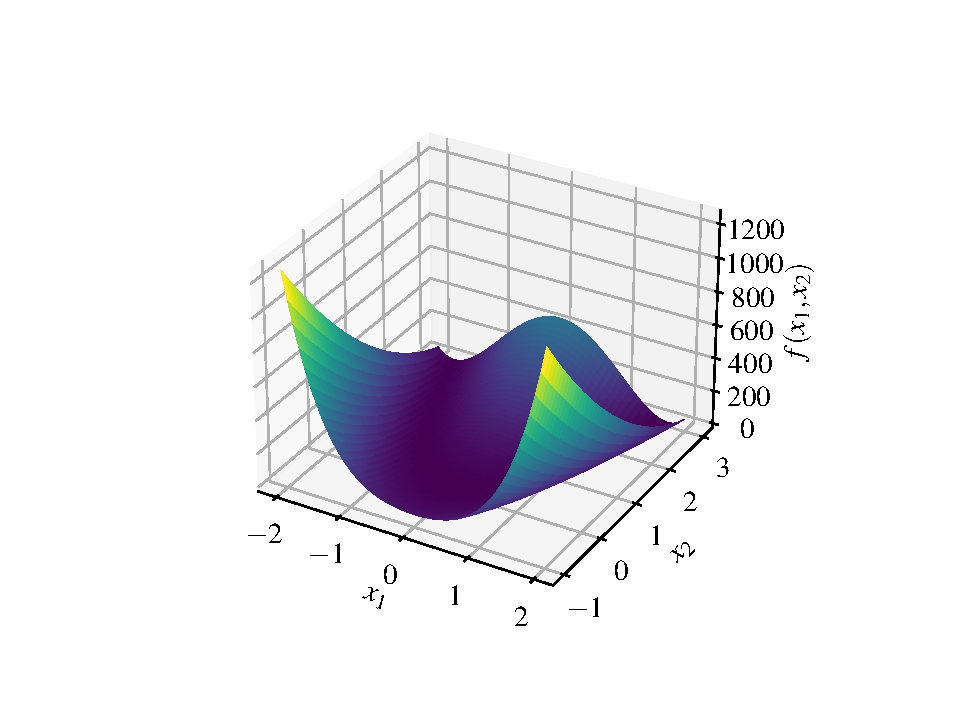
\includegraphics[width=0.5\textwidth]{figures/extended_rosenbrock_surf.pdf}
    \caption{Surface plot of the 2-dimensional extended Rosenbrock function}
    \label{fig:extended_rosenbrock_surf}
\end{figure}

\subsection{Exact gradient and Hessian}
\label{subsec:extended_rosenbrock_exact}

The gradient of the extended Rosenbrock function is given by the following expression,
\begin{equation}
    \frac{\partial F}{\partial x_k} = 
    \left \{ \begin{array}{ll}
    200(x_k^3 - x_kx_{k+1}) + (x_k - 1), & k\mod 2 = 1\\
    -100(x_{k-1}^2 - x_k), & k\mod 2 = 0
    \end{array} \right .
\end{equation}
computation can be eased considering that component $k$ depends only on $f_k$ and $f_{k+1}$ when $k$ is odd, and only on $f_{k-1}$ when $k$ is even.
The Hessian of the extended Rosenbrock function is given by the following expression.
\begin{equation}
    \frac{\partial^2 F}{\partial x_k \partial x_j} = 
    \left \{ \begin{array}{ll}
    200(3x_k^2 - x_{k+1}) + 1, & j = k,\ k\mod 2 = 1\\
    100, & j = k,\ k\mod 2 = 0\\
    -200x_k, & \lvert k-j \rvert = 1,\ k\mod 2 = 1\\
    0, & \text{otherwise}
    \end{array} \right .
\end{equation}
Notice that the Hessian is a sparse matrix, with only $n$ non-zero elements on the diagonal and $n/2$ non-zero elements on the first co-diagonal.

Table \ref{tab:Modified_Newton_Extended_Rosenbrock_exact} shows the results for the \textit{Modified Newton method} applied to the extended Rosenbrock function with exact gradient and Hessian.
All attempts were successful, and the method converged in a small number of iterations, with a convergence rate that is close to 2 for all dimensions but $10^5$, where the convergence rate is smaller and close to 1.
However, the time required to converge is significantly higher for the $10^5$-dimensional problem, which is expected due to the increased number of function evaluations required to compute the gradient and Hessian.
We observe that being the number of iterations necessary to converge to the minimum of the function very low, the experimental convergence rate is not very reliable, as it is computed as the ratio between the number of iterations and the logarithm of the relative error.

Table \ref{tab:Truncated_Newton_Extended_Rosenbrock_exact} shows the results for the \textit{Truncated Newton method} applied to the extended Rosenbrock function with exact gradient and Hessian.
All attempts were successful, and the method converged in a small number of iterations.
The computed experimental convergence rate is not reliable at all, presumably due to the small number of iterations and truncations of the iterative solver used to solve the Newton system.
Moreover, when preconditioning is not adopted we get a negative convergence rate since $\log \lVert e_k \rVert$ where $e_k$ is the error at iteration $k$ is not monotonic with respect to $k$, as shown in figure \ref{fig:extended_rosenbrock_error}.
However, when preconditioning is adopted and $k$ is larger, i.e. for $n = 10^5$, the convergence rate is superlinear as expected from the truncated Newton method with a superlinear forcing term.

Figure \ref{fig:extended_rosenbrock_error} shows the estimate of the error for the Modified Newton method and for the Truncated Newton method applied to the Extended Rosenbrock function with exact gradient and Hessian for $n=10^5$ when starting from random point 1:
\begin{itemize}
\item for the \textit{Modified Newton method}, in early iterates the estimated error is not monotonic, but it becomes monotonic after a few iterations regardless of preconditioning;
\item for the \textit{Truncated Newton method}, in early iterates the estimated error is not monotonic, but it becomes monotonic after a few iterations, but only if preconditioning is adopted.
\end{itemize}
Both in the case of the Modified Newton method and the Truncated Newton method, preconditioning improves performance of the optimization algorithms both in terms of number of iterations and time required to converge.

\begin{figure}
    \centering
    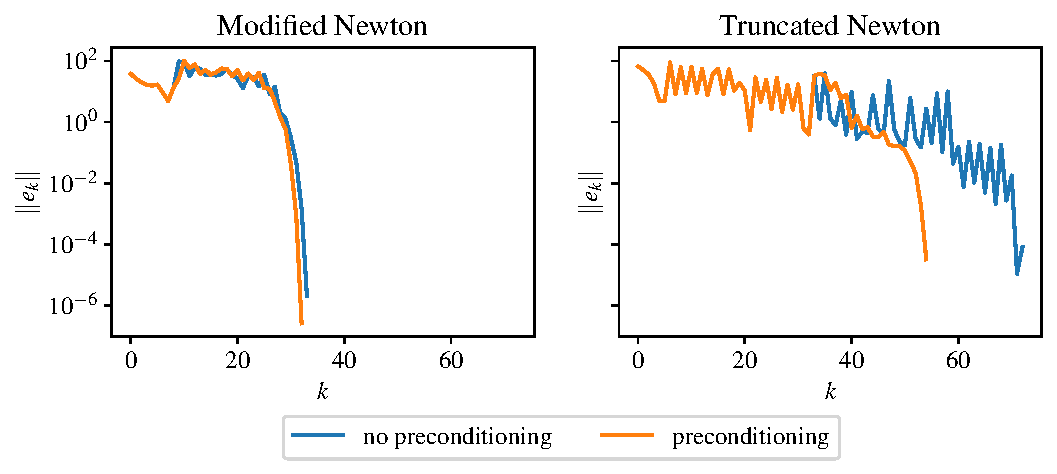
\includegraphics[width=0.75\textwidth]{figures/extended_rosenbrock_error.pdf}
    \caption{Estimate of the error for Modified Newton method and for the Truncated Newton method applied to the Extended Rosenbrock function with exact gradient and Hessian for $n=10^5$, random point 1.}
    \label{fig:extended_rosenbrock_error}
\end{figure}

\begin{table}
\centering
\caption{Results for Modified Newton method applied to Extended Rosenbrock with exact gradient and hessian, metrics are average metrics for succesful attempts.}
\label{tab:Modified_Newton_Extended_Rosenbrock_exact}
\begin{tabular}{r|cc|cc|cc|cc}
\toprule
    & \multicolumn{2}{|c}{iterations} & \multicolumn{2}{|c}{convergence rate} & \multicolumn{2}{|c}{time} & \multicolumn{2}{|c}{success rate} \\
preconditioning & False & True & False & True & False & True & False & True \\
dimension &  &  &  &  &  &  &  &  \\
\midrule
3 & 31.91 & 28.91 & 1.99 & 1.51 & 0.05 & 0.02 & 1.00 & 1.00 \\
4 & 32.36 & 29.18 & 2.10 & 2.04 & 0.11 & 0.08 & 1.00 & 1.00 \\
5 & 26.50 & 26.00 & 1.10 & 1.00 & 0.68 & 0.53 & 1.00 & 1.00 \\
\bottomrule
\end{tabular}
\end{table}

\begin{table}
\centering
\caption{Results for Truncated Newton method applied to Extended Rosenbrock with exact gradient and hessian, metrics are average metrics for succesful attempts.}
\label{tab:Truncated_Newton_Extended_Rosenbrock_exact}
\begin{tabular}{r|cc|cc|cc|cc}
\toprule
    & \multicolumn{2}{|c}{iterations} & \multicolumn{2}{|c}{convergence rate} & \multicolumn{2}{|c}{time} & \multicolumn{2}{|c}{success rate} \\
preconditioning & False & True & False & True & False & True & False & True \\
dimension &  &  &  &  &  &  &  &  \\
\midrule
3 & 50.09 & 31.00 & -2.66 & 11.55 & 0.01 & 0.01 & 1.00 & 1.00 \\
4 & 57.27 & 34.73 & -3.06 & 4.33 & 0.04 & 0.03 & 1.00 & 1.00 \\
5 & 64.00 & 28.50 & -5.58 & 1.62 & 0.45 & 0.23 & 1.00 & 1.00 \\
\bottomrule
\end{tabular}
\end{table}

\subsection{Finite differences gradient and Hessian}
\label{subsec:extended_rosenbrock_findiff}

When applying \ref{eq:findiff_gradient}, one can notice that the terms $F(x + he_k)$ and $F(x-he_k)$ only differ by terms $f_k$ and $f_{k+1}$ for $k$ odd, by terms $f_{k-1}$ for $k$ even.
Then to make function evaluations less expensive, we can define the following function $F_{\textit{fd},\,k}$, which can be plugged in \ref{eq:findiff_gradient} in place of $F$ yielding the same result.
\[
F_{\textit{fd},\,k}(x) = \left \{ \begin{array}{ll}
\frac12 f_k^2(x) + \frac12 f_{k+1}^2(x), & k\mod 2 = 1\\[.1cm]
\frac12 f_{k-1}^2(x), & k\mod 2 = 0
\end{array} \right .
\]
The same procedure can be applied for the Hessian, considering that:
\begin{itemize}
    \item function evaluations to compute entry $h_{k,k}$ differ only by $f_k$ and $f_{k+1}$ for $k$ odd, and only on $f_{k-1}$ for $k$ even;
    \item function evaluations to compute entry $h_{k,k+1}$ differ only by $f_k$ and $f_{k+1}$ for $k$ odd.
\end{itemize}
Then to make function evaluations less expensive, we can define the functions $F_{\textit{fd},\,k,k}$ and $F_{\textit{fd},\,k,k+1}$, which can be plugged in \ref{eq:findiff_hessian} in place of $F$ yielding the same result to compute entries $h_{k,k}$ and $h_{k,k+1}$ respectively.
\begin{align*}
F_{\textit{fd},\,k,k}(x) &= \left \{ \begin{array}{ll}
\frac12 f_k^2(x) + \frac12 f_{k+1}^2(x), & k\mod 2 = 1\\[.1cm]
\frac12 f_{k-1}^2(x), & k\mod 2 = 0
\end{array} \right .\\
F_{\textit{fd},\,k,k+1}(x) &= \left \{ \begin{array}{ll}
\frac12 f_k^2(x) + \frac12 f_{k+1}^2(x), & k\mod 2 = 1\\[.1cm]
0, & k\mod 2 = 0
\end{array} \right .
\end{align*}
When plugging the functions $F_{fd,\,k}$, $F_{\textit{fd},\,k,k}$ and $F_{\textit{fd},\,k,k+1}$ into \ref{eq:findiff_gradient} and \ref{eq:findiff_hessian} it's convenient to expand them so that the computation of the gradient and Hessian is not subject to numerical cancellation.
After expanding the functions, the gradient and Hessian can be approximated as follows.
\begin{align*}
    \frac{\partial F}{\partial x_k} &\approx \left \{ \begin{array}{ll}
        600h^2 x_k - 100hx_{k+1} + \frac12h + 350h^3 + 300hx_k^2, & k\mod 2 = 1\\
        -100x_{k-1}^2 + 100x_k, & k\mod 2 = 0
    \end{array} \right .\\
    \frac{\partial^2 F}{\partial x_k \partial x_j} &\approx \left \{ \begin{array}{ll}
        1200h_k x_k - 200x_{k+1} + 1 + 700h_k^2 + 600x_k^2, & j = k,\ k\mod 2 = 1\\
        100, & j = k,\ k\mod 2 = 0\\
        -100 h_k h_{k+1} - 200 x_k, & \lvert k-j \rvert = 1,\ k\mod 2 = 1\\
        0, & \text{otherwise}
    \end{array} \right .
\end{align*}

Tables \ref{tab:Modified_Newton_Extended_Rosenbrock_fd_abs} and \ref{tab:Modified_Newton_Extended_Rosenbrock_fd_rel} show the results for the \textit{Modified Newton method} applied to the extended Rosenbrock function with absolute and specific finite differences respectively.
All attempts were successful, and the method converged in a small number of iterations, with a convergence rate that is close to 2 for all dimensions, when a suitable choice of $h$ is made.
On the contrary, when a poor choice of $h$ is made, the convergence rate is close to 1, which is expected since the convergence rate of the Newton method is 2: this happens when $h=10^{-2}$ or $h=10^{-4}$, both for the constant increment and the specific increment methodologies.
We notice that for a fixed dimension, performance improves as the stepsize $h$ (be it constant or specific) decreases, as expected, up to a certain point where reducing the stepsize does not result in any improvement (i.e. time and iterations do not significantly decrease).
This plateau is reached sooner when preconditioning is adopted and when the dimension is lower.

\begin{table}
\centering
\caption{Results for Modified Newton method applied to Extended Rosenbrock with absolute finite differences, metrics are average metrics for succesful attempts.}
\label{tab:Modified_Newton_Extended_Rosenbrock_fd_abs}
\begin{tabular}{rr|cc|cc|cc|cc}
\toprule
    &  & \multicolumn{2}{|c}{iterations} & \multicolumn{2}{|c}{convergence rate} & \multicolumn{2}{|c}{time} & \multicolumn{2}{|c}{success rate} \\
    & preconditioning & False & True & False & True & False & True & False & True \\
dimension & h &  &  &  &  &  &  &  &  \\
\midrule
\multirow[t]{6}{*}{3} & 1e-02 & 149.91 & 150.82 & 1.00 & 1.00 & 0.07 & 0.07 & 1.00 & 1.00 \\
    & 1e-04 & 33.18 & 32.09 & 1.01 & 1.00 & 0.02 & 0.02 & 1.00 & 1.00 \\
    & 1e-06 & 32.09 & 30.18 & 1.96 & 2.09 & 0.03 & 0.02 & 1.00 & 1.00 \\
    & 1e-08 & 32.00 & 30.18 & 2.04 & 2.23 & 0.02 & 0.02 & 1.00 & 1.00 \\
    & 1e-10 & 32.00 & 30.18 & 2.00 & 2.23 & 0.02 & 0.02 & 1.00 & 1.00 \\
    & 1e-12 & 32.00 & 30.18 & 2.00 & 2.23 & 0.02 & 0.02 & 1.00 & 1.00 \\
\cline{1-10}
\multirow[t]{6}{*}{4} & 1e-02 & 160.09 & 160.55 & 1.00 & 1.00 & 0.34 & 0.36 & 1.00 & 1.00 \\
    & 1e-04 & 34.18 & 32.55 & 1.00 & 1.00 & 0.12 & 0.09 & 1.00 & 1.00 \\
    & 1e-06 & 32.55 & 30.27 & 1.89 & 1.96 & 0.12 & 0.08 & 1.00 & 1.00 \\
    & 1e-08 & 32.55 & 30.27 & 1.95 & 1.98 & 0.12 & 0.08 & 1.00 & 1.00 \\
    & 1e-10 & 32.55 & 30.27 & 1.95 & 1.98 & 0.11 & 0.08 & 1.00 & 1.00 \\
    & 1e-12 & 32.55 & 30.27 & 1.95 & 1.98 & 0.11 & 0.08 & 1.00 & 1.00 \\
\cline{1-10}
\multirow[t]{6}{*}{5} & 1e-02 & 169.36 & 169.82 & 1.00 & 1.00 & 3.26 & 3.36 & 1.00 & 1.00 \\
    & 1e-04 & 34.82 & 33.73 & 1.00 & 1.00 & 1.08 & 0.79 & 1.00 & 1.00 \\
    & 1e-06 & 34.00 & 31.73 & 2.13 & 2.00 & 1.17 & 0.75 & 1.00 & 1.00 \\
    & 1e-08 & 33.27 & 31.73 & 2.60 & 2.10 & 1.17 & 0.73 & 1.00 & 1.00 \\
    & 1e-10 & 33.45 & 31.73 & 1.93 & 2.10 & 1.13 & 0.73 & 1.00 & 1.00 \\
    & 1e-12 & 33.45 & 31.73 & 1.90 & 2.10 & 1.15 & 0.73 & 1.00 & 1.00 \\
\cline{1-10}
\bottomrule
\end{tabular}
\end{table}

\begin{table}
\centering
\caption{Results for Modified Newton method applied to Extended Rosenbrock with specific finite differences, metrics are average metrics for succesful attempts.}
\label{tab:Modified_Newton_Extended_Rosenbrock_fd_rel}
\begin{tabular}{rr|cc|cc|cc|cc}
\toprule
    &  & \multicolumn{2}{|c}{iterations} & \multicolumn{2}{|c}{convergence rate} & \multicolumn{2}{|c}{time} & \multicolumn{2}{|c}{success rate} \\
    & preconditioning & False & True & False & True & False & True & False & True \\
dimension & h &  &  &  &  &  &  &  &  \\
\midrule
\multirow[t]{6}{*}{3} & 1e-02 & 139.82 & 141.45 & 1.00 & 1.00 & 0.06 & 0.06 & 1.00 & 1.00 \\
    & 1e-04 & 33.73 & 32.27 & 1.00 & 1.00 & 0.02 & 0.02 & 1.00 & 1.00 \\
    & 1e-06 & 32.09 & 30.18 & 1.89 & 2.06 & 0.02 & 0.02 & 1.00 & 1.00 \\
    & 1e-08 & 32.00 & 30.18 & 2.04 & 2.23 & 0.02 & 0.02 & 1.00 & 1.00 \\
    & 1e-10 & 32.00 & 30.18 & 2.00 & 2.23 & 0.02 & 0.02 & 1.00 & 1.00 \\
    & 1e-12 & 32.00 & 30.18 & 2.00 & 2.23 & 0.02 & 0.02 & 1.00 & 1.00 \\
\cline{1-10}
\multirow[t]{6}{*}{4} & 1e-02 & 149.55 & 150.55 & 1.00 & 1.00 & 0.32 & 0.32 & 1.00 & 1.00 \\
    & 1e-04 & 34.45 & 32.45 & 1.00 & 1.00 & 0.12 & 0.09 & 1.00 & 1.00 \\
    & 1e-06 & 32.55 & 30.27 & 1.81 & 1.96 & 0.12 & 0.09 & 1.00 & 1.00 \\
    & 1e-08 & 32.55 & 30.27 & 1.95 & 1.98 & 0.12 & 0.08 & 1.00 & 1.00 \\
    & 1e-10 & 32.55 & 30.27 & 1.95 & 1.98 & 0.12 & 0.08 & 1.00 & 1.00 \\
    & 1e-12 & 32.55 & 30.27 & 1.95 & 1.98 & 0.11 & 0.08 & 1.00 & 1.00 \\
\cline{1-10}
\multirow[t]{6}{*}{5} & 1e-02 & 159.18 & 160.27 & 1.00 & 1.00 & 3.05 & 3.17 & 1.00 & 1.00 \\
    & 1e-04 & 34.64 & 34.45 & 1.00 & 1.00 & 1.09 & 0.80 & 1.00 & 1.00 \\
    & 1e-06 & 33.45 & 31.73 & 2.56 & 2.00 & 1.16 & 0.74 & 1.00 & 1.00 \\
    & 1e-08 & 33.09 & 31.73 & 1.84 & 2.10 & 1.13 & 0.73 & 1.00 & 1.00 \\
    & 1e-10 & 33.45 & 31.73 & 1.90 & 2.10 & 1.12 & 0.74 & 1.00 & 1.00 \\
    & 1e-12 & 33.45 & 31.73 & 1.90 & 2.10 & 1.14 & 0.77 & 1.00 & 1.00 \\
\cline{1-10}
\bottomrule
\end{tabular}
\end{table}

Tables \ref{tab:Truncated_Newton_Extended_Rosenbrock_fd_abs} and \ref{tab:Truncated_Newton_Extended_Rosenbrock_fd_rel} show the results for the \textit{Truncated Newton method} applied to the extended Rosenbrock function with absolute and specific finite differences respectively.
All attempts were successful, and the method converged in a small number of iterations, when a suitable choice of $h$ is made.
A larger number of iterations is required when a poor choice of $h$ is made, namely when $h=10^{-2}$ or $h=10^{-4}$, both for the constant increment and the specific increment methodologies, yielding a convergence rate of 1.
For smaller values of $h$, the estimate of the convergence rate is not reliable at all and considerations made in subsection \ref{subsec:extended_rosenbrock_exact} for the Truncated Newton method applied to the extended Rosenbrock function with exact gradient and Hessian apply here as well.
The plateau in performance as the stepsize $h$ decreases is reached slower than in the case of the Modified Newton method, hinting that the Truncated Newton method highly benefits from a finer approximation of the derivatives.

\begin{table}
\centering
\caption{Results for Truncated Newton method applied to Extended Rosenbrock with absolute finite differences, metrics are average metrics for succesful attempts.}
\label{tab:Truncated_Newton_Extended_Rosenbrock_fd_abs}
\begin{tabular}{rr|cc|cc|cc|cc}
\toprule
    &  & \multicolumn{2}{|c}{iterations} & \multicolumn{2}{|c}{convergence rate} & \multicolumn{2}{|c}{time} & \multicolumn{2}{|c}{success rate} \\
    & preconditioning & False & True & False & True & False & True & False & True \\
dimension & h &  &  &  &  &  &  &  &  \\
\midrule
\multirow[t]{6}{*}{3} & 1e-02 & 182.00 & 179.27 & 1.00 & 1.00 & 0.02 & 0.04 & 1.00 & 1.00 \\
    & 1e-04 & 54.36 & 37.91 & 1.00 & 1.00 & 0.01 & 0.01 & 1.00 & 1.00 \\
    & 1e-06 & 52.82 & 36.36 & -1.48 & 2.39 & 0.01 & 0.01 & 1.00 & 1.00 \\
    & 1e-08 & 52.91 & 35.91 & -2.12 & 2.86 & 0.01 & 0.01 & 1.00 & 1.00 \\
    & 1e-10 & 53.36 & 35.45 & -4.10 & 2.21 & 0.01 & 0.01 & 1.00 & 1.00 \\
    & 1e-12 & 55.64 & 36.45 & -2.49 & 3.01 & 0.01 & 0.01 & 1.00 & 1.00 \\
\cline{1-10}
\multirow[t]{6}{*}{4} & 1e-02 & 203.91 & 192.18 & 1.00 & 1.00 & 0.16 & 0.17 & 1.00 & 1.00 \\
    & 1e-04 & 61.64 & 44.45 & 1.00 & 1.00 & 0.06 & 0.05 & 1.00 & 1.00 \\
    & 1e-06 & 59.18 & 42.55 & -1.35 & 4.36 & 0.06 & 0.05 & 1.00 & 1.00 \\
    & 1e-08 & 61.64 & 42.09 & -1.78 & 2.34 & 0.06 & 0.05 & 1.00 & 1.00 \\
    & 1e-10 & 62.27 & 41.91 & -2.46 & 3.14 & 0.06 & 0.05 & 1.00 & 1.00 \\
    & 1e-12 & 61.73 & 43.00 & -2.89 & 2.65 & 0.06 & 0.05 & 1.00 & 1.00 \\
\cline{1-10}
\multirow[t]{6}{*}{5} & 1e-02 & 224.55 & 206.82 & 1.00 & 1.00 & 1.84 & 1.83 & 1.00 & 1.00 \\
    & 1e-04 & 74.64 & 42.91 & 1.00 & 1.01 & 0.73 & 0.41 & 1.00 & 1.00 \\
    & 1e-06 & 79.09 & 49.27 & -2.17 & 2.06 & 0.81 & 0.50 & 1.00 & 1.00 \\
    & 1e-08 & 75.64 & 49.91 & -2.83 & 7.31 & 0.75 & 0.47 & 1.00 & 1.00 \\
    & 1e-10 & 78.00 & 51.64 & -1.21 & 3.21 & 0.75 & 0.50 & 1.00 & 1.00 \\
    & 1e-12 & 78.00 & 53.27 & -2.11 & 2.50 & 0.77 & 0.52 & 1.00 & 1.00 \\
\cline{1-10}
\bottomrule
\end{tabular}
\end{table}

\begin{table}
\centering
\caption{Results for Truncated Newton method applied to Extended Rosenbrock with specific finite differences, metrics are average metrics for succesful attempts.}
\label{tab:Truncated_Newton_Extended_Rosenbrock_fd_rel}
\begin{tabular}{rr|cc|cc|cc|cc}
\toprule
    &  & \multicolumn{2}{|c}{iterations} & \multicolumn{2}{|c}{convergence rate} & \multicolumn{2}{|c}{time} & \multicolumn{2}{|c}{success rate} \\
    & preconditioning & False & True & False & True & False & True & False & True \\
dimension & h &  &  &  &  &  &  &  &  \\
\midrule
\multirow[t]{6}{*}{3} & 1e-02 & 169.91 & 169.91 & 1.00 & 1.00 & 0.02 & 0.03 & 1.00 & 1.00 \\
    & 1e-04 & 54.45 & 37.27 & 1.00 & 1.02 & 0.01 & 0.01 & 1.00 & 1.00 \\
    & 1e-06 & 51.45 & 36.27 & -2.69 & 2.35 & 0.01 & 0.01 & 1.00 & 1.00 \\
    & 1e-08 & 53.64 & 36.27 & -3.43 & 1.91 & 0.01 & 0.01 & 1.00 & 1.00 \\
    & 1e-10 & 54.64 & 35.27 & -2.94 & 2.01 & 0.01 & 0.01 & 1.00 & 1.00 \\
    & 1e-12 & 53.82 & 35.91 & -4.18 & 2.56 & 0.01 & 0.01 & 1.00 & 1.00 \\
\cline{1-10}
\multirow[t]{6}{*}{4} & 1e-02 & 191.09 & 182.64 & 1.00 & 1.00 & 0.15 & 0.17 & 1.00 & 1.00 \\
    & 1e-04 & 64.27 & 42.55 & 1.00 & 1.01 & 0.06 & 0.05 & 1.00 & 1.00 \\
    & 1e-06 & 62.18 & 43.00 & -0.96 & 2.62 & 0.06 & 0.05 & 1.00 & 1.00 \\
    & 1e-08 & 60.73 & 40.91 & -2.95 & 2.87 & 0.06 & 0.05 & 1.00 & 1.00 \\
    & 1e-10 & 60.82 & 42.73 & -1.22 & 3.98 & 0.06 & 0.05 & 1.00 & 1.00 \\
    & 1e-12 & 63.09 & 42.91 & -2.01 & 2.51 & 0.06 & 0.05 & 1.00 & 1.00 \\
\cline{1-10}
\multirow[t]{6}{*}{5} & 1e-02 & 213.55 & 198.64 & 1.00 & 1.00 & 1.68 & 1.74 & 1.00 & 1.00 \\
    & 1e-04 & 75.91 & 40.82 & 1.00 & 1.00 & 0.74 & 0.42 & 1.00 & 1.00 \\
    & 1e-06 & 77.91 & 49.00 & -2.96 & 6.91 & 0.77 & 0.49 & 1.00 & 1.00 \\
    & 1e-08 & 77.64 & 50.18 & -1.96 & 2.28 & 0.77 & 0.48 & 1.00 & 1.00 \\
    & 1e-10 & 75.00 & 53.27 & -4.07 & 3.38 & 0.75 & 0.52 & 1.00 & 1.00 \\
    & 1e-12 & 75.09 & 52.45 & -2.09 & 3.48 & 0.75 & 0.52 & 1.00 & 1.00 \\
\cline{1-10}
\bottomrule
\end{tabular}
\end{table}
